\documentclass{standalone}
\usepackage{tikz}
\usetikzlibrary{patterns, positioning}

\begin{document}
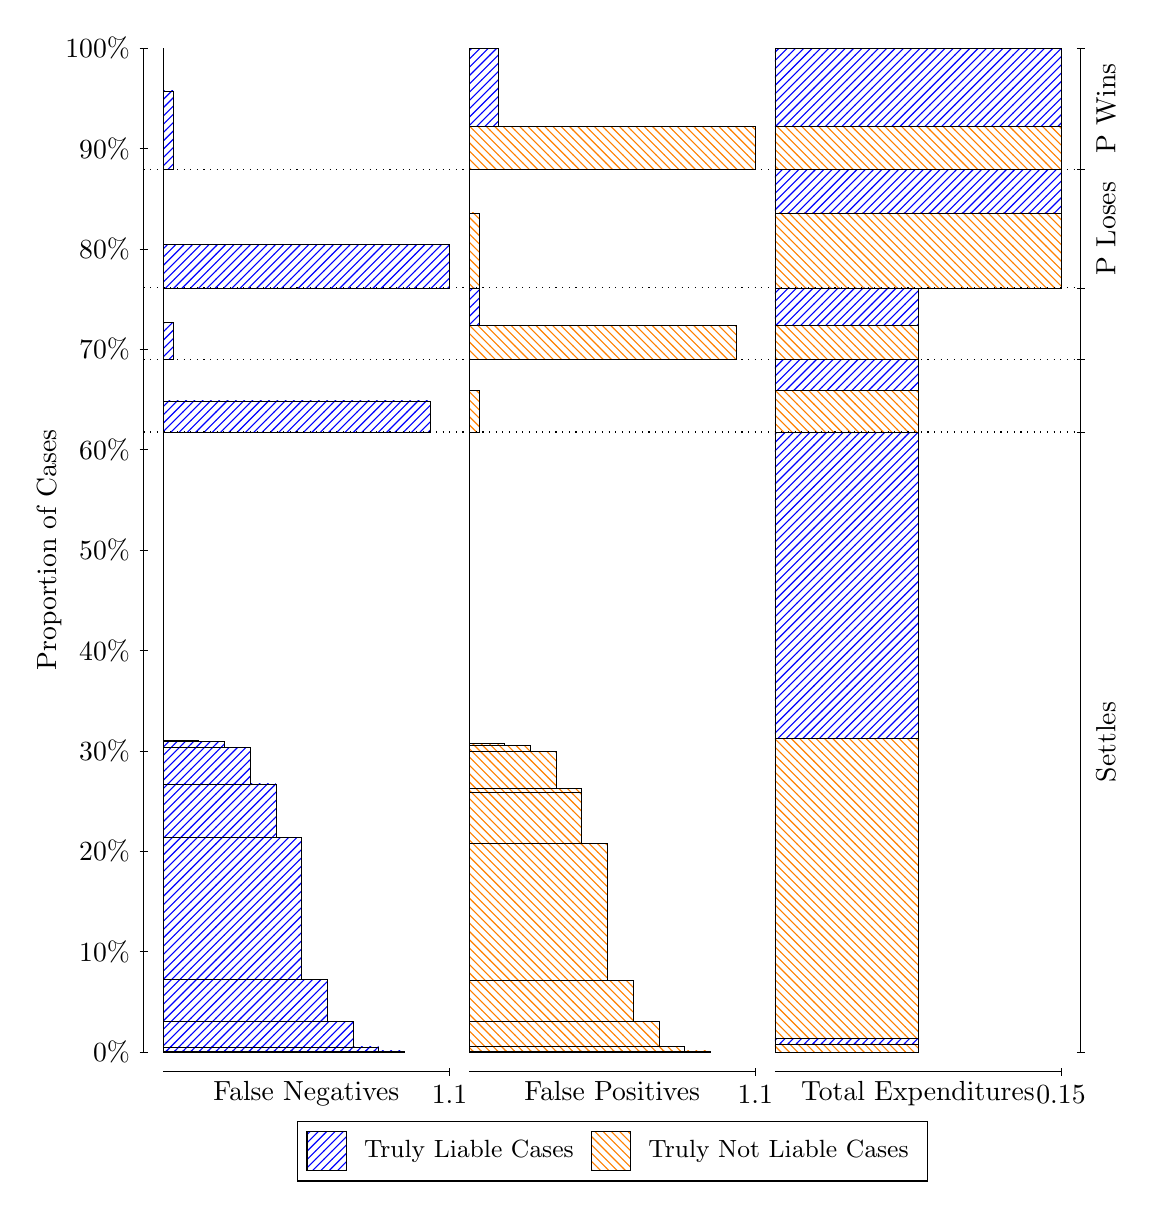
\begin{tikzpicture}
\draw[black, very thin] (1.5,1.75) -- (1.5,14.5);
\node[rotate=90, anchor=center] at (0.3, 8.125) {Proportion of Cases};
\draw[black, very thin] (1.45,1.75) -- (1.55,1.75);
\node[anchor=east] at (1.45, 1.75) {0\%};
\draw[black, very thin] (1.45,3.025) -- (1.55,3.025);
\node[anchor=east] at (1.45, 3.025) {10\%};
\draw[black, very thin] (1.45,4.3) -- (1.55,4.3);
\node[anchor=east] at (1.45, 4.3) {20\%};
\draw[black, very thin] (1.45,5.575) -- (1.55,5.575);
\node[anchor=east] at (1.45, 5.575) {30\%};
\draw[black, very thin] (1.45,6.85) -- (1.55,6.85);
\node[anchor=east] at (1.45, 6.85) {40\%};
\draw[black, very thin] (1.45,8.125) -- (1.55,8.125);
\node[anchor=east] at (1.45, 8.125) {50\%};
\draw[black, very thin] (1.45,9.4) -- (1.55,9.4);
\node[anchor=east] at (1.45, 9.4) {60\%};
\draw[black, very thin] (1.45,10.675) -- (1.55,10.675);
\node[anchor=east] at (1.45, 10.675) {70\%};
\draw[black, very thin] (1.45,11.95) -- (1.55,11.95);
\node[anchor=east] at (1.45, 11.95) {80\%};
\draw[black, very thin] (1.45,13.225) -- (1.55,13.225);
\node[anchor=east] at (1.45, 13.225) {90\%};
\draw[black, very thin] (1.45,14.5) -- (1.55,14.5);
\node[anchor=east] at (1.45, 14.5) {100\%};

\draw[black, very thin] (13.4,1.75) -- (13.4,14.5);
\draw[black, very thin] (13.35,1.75) -- (13.45,1.75);
\node[anchor=west] at (13.35, 1.75) {};
\draw[black, very thin] (13.35,9.6235) -- (13.45,9.6235);
\node[anchor=west] at (13.35, 9.6235) {};
\draw[black, very thin] (13.35,10.547) -- (13.45,10.547);
\node[anchor=west] at (13.35, 10.547) {};
\draw[black, very thin] (13.35,11.454) -- (13.45,11.454);
\node[anchor=west] at (13.35, 11.454) {};
\draw[black, very thin] (13.35,12.963) -- (13.45,12.963);
\node[anchor=west] at (13.35, 12.963) {};
\draw[black, very thin] (13.35,14.5) -- (13.45,14.5);
\node[anchor=west] at (13.35, 14.5) {};

\draw[black, very thin, pattern color=blue, pattern=north east lines] (1.75,1.75) rectangle (4.8118,1.7652);
\draw[black, very thin, pattern color=blue, pattern=north east lines] (1.75,1.7652) rectangle (4.4852,1.816);
\draw[black, very thin, pattern color=blue, pattern=north east lines] (1.75,1.816) rectangle (4.1586,2.1384);
\draw[black, very thin, pattern color=blue, pattern=north east lines] (1.75,2.1384) rectangle (3.832,2.676);
\draw[black, very thin, pattern color=blue, pattern=north east lines] (1.75,2.676) rectangle (3.5054,4.4781);
\draw[black, very thin, pattern color=blue, pattern=north east lines] (1.75,4.4781) rectangle (3.1788,5.1536);
\draw[black, very thin, pattern color=blue, pattern=north east lines] (1.75,5.1536) rectangle (2.8522,5.6174);
\draw[black, very thin, pattern color=blue, pattern=north east lines] (1.75,5.6174) rectangle (2.5257,5.6904);
\draw[black, very thin, pattern color=blue, pattern=north east lines] (1.75,5.6904) rectangle (2.1991,5.7065);
\draw[black, very thin, pattern color=orange, pattern=north west lines] (1.75,5.7065) rectangle (1.75,9.6235);
\draw[black, very thin, pattern color=blue, pattern=north east lines] (1.75,9.6235) rectangle (5.1384,10.02);
\draw[black, very thin, pattern color=orange, pattern=north west lines] (1.75,10.02) rectangle (1.75,10.547);
\draw[black, very thin, pattern color=blue, pattern=north east lines] (1.75,10.547) rectangle (1.8725,11.018);
\draw[black, very thin, pattern color=orange, pattern=north west lines] (1.75,11.018) rectangle (1.75,11.454);
\draw[black, very thin, pattern color=blue, pattern=north east lines] (1.75,11.454) rectangle (5.3833,12.011);
\draw[black, very thin, pattern color=orange, pattern=north west lines] (1.75,12.011) rectangle (1.75,12.963);
\draw[black, very thin, pattern color=blue, pattern=north east lines] (1.75,12.963) rectangle (1.8725,13.957);
\draw[black, very thin, pattern color=orange, pattern=north west lines] (1.75,13.957) rectangle (1.75,14.5);
\draw[black, very thin, pattern color=orange, pattern=north west lines] (5.6333,1.75) rectangle (8.6951,1.7648);
\draw[black, very thin, pattern color=orange, pattern=north west lines] (5.6333,1.7648) rectangle (8.3685,1.8182);
\draw[black, very thin, pattern color=orange, pattern=north west lines] (5.6333,1.8182) rectangle (8.0419,2.1409);
\draw[black, very thin, pattern color=orange, pattern=north west lines] (5.6333,2.1409) rectangle (7.7154,2.6564);
\draw[black, very thin, pattern color=orange, pattern=north west lines] (5.6333,2.6564) rectangle (7.3888,4.4031);
\draw[black, very thin, pattern color=orange, pattern=north west lines] (5.6333,4.4031) rectangle (7.0622,5.0455);
\draw[black, very thin, pattern color=orange, pattern=north west lines] (5.6333,5.0455) rectangle (7.0622,5.0928);
\draw[black, very thin, pattern color=orange, pattern=north west lines] (5.6333,5.0928) rectangle (6.7356,5.5645);
\draw[black, very thin, pattern color=orange, pattern=north west lines] (5.6333,5.5645) rectangle (6.409,5.6423);
\draw[black, very thin, pattern color=orange, pattern=north west lines] (5.6333,5.6423) rectangle (6.0824,5.667);
\draw[black, very thin, pattern color=blue, pattern=north east lines] (5.6333,5.667) rectangle (5.6333,9.6235);
\draw[black, very thin, pattern color=orange, pattern=north west lines] (5.6333,9.6235) rectangle (5.7558,10.15);
\draw[black, very thin, pattern color=blue, pattern=north east lines] (5.6333,10.15) rectangle (5.6333,10.547);
\draw[black, very thin, pattern color=orange, pattern=north west lines] (5.6333,10.547) rectangle (9.0217,10.982);
\draw[black, very thin, pattern color=blue, pattern=north east lines] (5.6333,10.982) rectangle (5.7558,11.454);
\draw[black, very thin, pattern color=orange, pattern=north west lines] (5.6333,11.454) rectangle (5.7558,12.406);
\draw[black, very thin, pattern color=blue, pattern=north east lines] (5.6333,12.406) rectangle (5.6333,12.963);
\draw[black, very thin, pattern color=orange, pattern=north west lines] (5.6333,12.963) rectangle (9.2667,13.506);
\draw[black, very thin, pattern color=blue, pattern=north east lines] (5.6333,13.506) rectangle (6.0007,14.5);
\draw[black, very thin, pattern color=orange, pattern=north west lines] (9.5167,1.75) rectangle (11.333,1.8525);
\draw[black, very thin, pattern color=blue, pattern=north east lines] (9.5167,1.8525) rectangle (11.333,1.9185);
\draw[black, very thin, pattern color=orange, pattern=north west lines] (9.5167,1.9185) rectangle (11.333,5.733);
\draw[black, very thin, pattern color=blue, pattern=north east lines] (9.5167,5.733) rectangle (11.333,9.6235);
\draw[black, very thin, pattern color=orange, pattern=north west lines] (9.5167,9.6235) rectangle (11.333,10.15);
\draw[black, very thin, pattern color=blue, pattern=north east lines] (9.5167,10.15) rectangle (11.333,10.547);
\draw[black, very thin, pattern color=orange, pattern=north west lines] (9.5167,10.547) rectangle (11.333,10.982);
\draw[black, very thin, pattern color=blue, pattern=north east lines] (9.5167,10.982) rectangle (11.333,11.454);
\draw[black, very thin, pattern color=orange, pattern=north west lines] (9.5167,11.454) rectangle (13.15,12.406);
\draw[black, very thin, pattern color=blue, pattern=north east lines] (9.5167,12.406) rectangle (13.15,12.963);
\draw[black, very thin, pattern color=orange, pattern=north west lines] (9.5167,12.963) rectangle (13.15,13.506);
\draw[black, very thin, pattern color=blue, pattern=north east lines] (9.5167,13.506) rectangle (13.15,14.5);
\draw[black, dotted] (1.5,9.6235) -- (13.4,9.6235);
\draw[black, dotted] (1.5,10.547) -- (13.4,10.547);
\draw[black, dotted] (1.5,11.454) -- (13.4,11.454);
\draw[black, dotted] (1.5,12.963) -- (13.4,12.963);
\draw[black, very thin] (1.75,1.5) -- (5.3833,1.5);
\node[anchor=north] at (3.5667, 1.5) {False Negatives};
\draw[black, very thin] (5.3833,1.45) -- (5.3833,1.55);
\node[anchor=north] at (5.3833, 1.45) {1.1};

\draw[black, very thin] (5.6333,1.5) -- (9.2667,1.5);
\node[anchor=north] at (7.45, 1.5) {False Positives};
\draw[black, very thin] (9.2667,1.45) -- (9.2667,1.55);
\node[anchor=north] at (9.2667, 1.45) {1.1};

\draw[black, very thin] (9.5167,1.5) -- (13.15,1.5);
\node[anchor=north] at (11.333, 1.5) {Total Expenditures};
\draw[black, very thin] (13.15,1.45) -- (13.15,1.55);
\node[anchor=north] at (13.15, 1.45) {0.15};

\node[black, centered, rotate=90] at (13.72, 5.6867) {Settles};


\node[black, centered, rotate=90] at (13.72, 12.208) {P Loses};
\node[black, centered, rotate=90] at (13.72, 13.731) {P Wins};

\draw (7.449999999999999,1.5) node[draw=none] (baseCoordinate) {};
\begin{scope}[align=center]
        \matrix[scale=0.5, draw=black, below=0.5cm of baseCoordinate, nodes={draw}, column sep=0.1cm]{
            \node[rectangle, draw, minimum width=0.5cm, minimum height=0.5cm, pattern=north east lines, pattern color=blue] {}; &
            \node[draw=none, font=\small] (B) {Truly Liable Cases}; &
            \node[rectangle, draw, minimum width=0.5cm, minimum height=0.5cm, pattern=north west lines, pattern color=orange] {}; &
            \node[draw=none, font=\small] (B) {Truly Not Liable Cases}; \\
            };
\end{scope}

\end{tikzpicture}
\end{document}